\documentclass[11pt]{article}
\setlength{\parskip}{10pt plus 1pt minus 1pt}
% For unindented paragraphs
\setlength{\parindent}{0em}
% For indented paragraphs
% \setlength{\parindent}{1em}
\usepackage[margin=1.25in]{geometry}
% No page numbers
%\pagestyle{empty}
% Page numbering
 \pagestyle{plain}

\newcommand{\textnum}[1]{\ensuremath{\mathmyrm{#1}}}
\newcommand{\dgr}{\boldmath\ensuremath{{}^\circ}\unboldmath}
\newcommand{\vlm}{V \!\!\!\!\!\!\: \rule[0.07in]{.095in}{.0025in}}

%%%%%%%%%%%%%%%%%%%%%%   Font choice   %%%%%%%%%%%%%%%%%%%%%%%%%
% Times-Roman
\renewcommand\familydefault{ptm}
\DeclareMathAlphabet{\mathmyrm}{OT1}{ptm}{m}{n}
\DeclareMathAlphabet{\mathmybf}{OT1}{ptm}{bx}{n}
\SetMathAlphabet{\mathmyrm}{bold}{OT1}{ptm}{bx}{n}
%%%%%%%%%%%%%%%%%%%%%%   Font choice (end)    %%%%%%%%%%%%%%%%%%%%

%%%%%%%%%%%%%%%%%%%%%%   Figures   %%%%%%%%%%%%%%%%%%%%%%%%%%%
\usepackage{graphicx}
%\includegraphics[width=2in]{couette}

% Subfig packages allows tiling of multiple figures into a single
% figure
\usepackage{subfig}
% Example:
% \begin{figure}
%   \centering
%   \subfloat[short caption a]{\label{fig:subA}\includegraphics[width=3.25in]{t49n283}} 
%   \subfloat[short caption b]{\label{fig:subB}\includegraphics[width=3.25in]{t49n328}} \\
%   \subfloat[short caption c]{\label{fig:subC}\includegraphics[width=3.25in]{t49n525}}
%   \subfloat[short caption d]{\label{fig:subD}\includegraphics[width=3.25in]{t49n635}} 
%   \caption{Overall caption for full figure}
%   \label{fig:t49}
% \end{figure}


% forces all figures in the section they are specified in
\usepackage[section]{placeins}

%%%%%%%%%%%%%%%%%%%%%%   Figures (end)   %%%%%%%%%%%%%%%%%%%%%%%

%%%%%%%%%%%%%%%%%%%%%%   Tables   %%%%%%%%%%%%%%%%%%%%%%%%%%%
\usepackage{booktabs}
\usepackage{multirow}
\newcommand{\ra}[1]{\renewcommand{\arraystretch}{#1}}
% More space between rows (this goes after \begin{table}):
%\renewcommand{\arraystretch}{1.2} % or 1.3
% or equivalently
% \ra{1.2}
% Remove space to the vertical edges:
% \begin{tabular}{@{}lll@{}}
% Three lines
% \toprule
% \midrule
% \bottomrule
% and if you need lines for partial columns
% cmidrule{3-5}
%%%%%%%%%%%%%%%%%%%%%%   Tables (end)   %%%%%%%%%%%%%%%%%%%%%%%

%%%%%%%%%%%%%%%%%%%%%%   Hyperlinking    %%%%%%%%%%%%%%%%%%%%%%%
\usepackage[colorlinks=true]{hyperref}
\hypersetup{linkcolor=blue, citecolor=blue, filecolor=blue, urlcolor=blue}
% If you just want to use the default colors, comment the line above
% For reference, the default is
%   linkcolor red          Color for normal internal links.
%   anchorcolor      black  Color for anchor text.
%   citecolor green Color for bibliographical citations in text.
%   filecolor  cyan   Color for URLs which open local files.
%   urlcolor   magenta       Color for linked URLs.
%%%%%%%%%%%%%%%%%%    Hyperlinking (end)  %%%%%%%%%%%%%%%%%%%%%%%%%


%%%%%%%%%%%%%%%%%%%%%%    Other        %%%%%%%%%%%%%%%%%%%%%%%%%%%%

% some additional symbols
\usepackage{latexsym}
\usepackage{amsmath,amssymb,amsfonts,textcomp}
\usepackage{morefloats}
%%%%%%%%%%%%%%%%%%%%%%    Other (end)  %%%%%%%%%%%%%%%%%%%%%%%%%%%%


%Title block -- put you information here
\title{Fluids Momentum}
\author{Team 2} % or anonymous paper ID number if
                          % appropriate
\date{\today} % or some other date if you would like


\begin{document}
\maketitle
% Comment out the next two lines if you are not including an abstract
% \begin{abstract}
  
% \end{abstract}

% Professional-looking not-quite-single-spacing
%\setlength{\baselineskip}{13pt}
% Double-spacing
\setlength{\baselineskip}{22pt}
%
% Start document below this line


\section{Results and Discussion}
The measured and theoretical data collectively describe the relationship between the reaction force and the independent variables investigated within the model given the identified uncertainties. These relationships can be illustrated by examining the trends between force, volume flow rate, nozzle diameter, angle of contact, and uncertainties. Most trends were identified by using least square regression power law curve fit which reflects the relationship $F\propto \dot{\vlm}^2$. Standard deviation and calculated uncertainties (Eq. 7-9) were used to find approximate error and verify that measured data supports theoretical data.


\subsection{Force vs Volume Flow rate}
The measured data featured in Figure 1 demonstrates that Force the fluid applied increases with the volumetric flow rate. The data also demonstrates that the relationship is not linear either. A power law curve fit function was utilized  with $scipi.optimize.curve\_fit$ tool to find the best fitting coefficients that represent the measured data. This provides a fair approximation as the data often lies within the error bars. The error bars take into account the standard deviation of the measurements, and the uncertainty of the force measuring device. The power law fit is potentially representative of the power-law relationship that exists in Eq. 9 stating that $F\propto V^2$.

A quantitative analysis and comparison with measured and modeled trends suggests that the model is useful in predicting the force that results from varied volumetric flow rate. Uncertainty for each of the instruments was considered to fully represent the datas (Table 2) nature and how accurate and  reasonable the data was that the test rig provided.Table 1 features all of the coefficients from each of the power law curve fits for each of the test scenarios. Note that that these power law relationships are approximately 2 once again supporting that the $F\propto V^2$ in Eq. 9. Figure 2 shows the model for each angle nozzle and volumetric flow rate combination. The models of course feature a power law curve, but also results that approximate the measured data. Figure 3 provides a side-by-side comparison of the 3.28 Nozzle with the modeled data and measured data. While the curves are similar, there are many cases in which the measured data lies outside of the error bars in the model.



 \begin{figure}
   \centering
   \subfloat[2.83mm nozzle]{\label{fig:subA}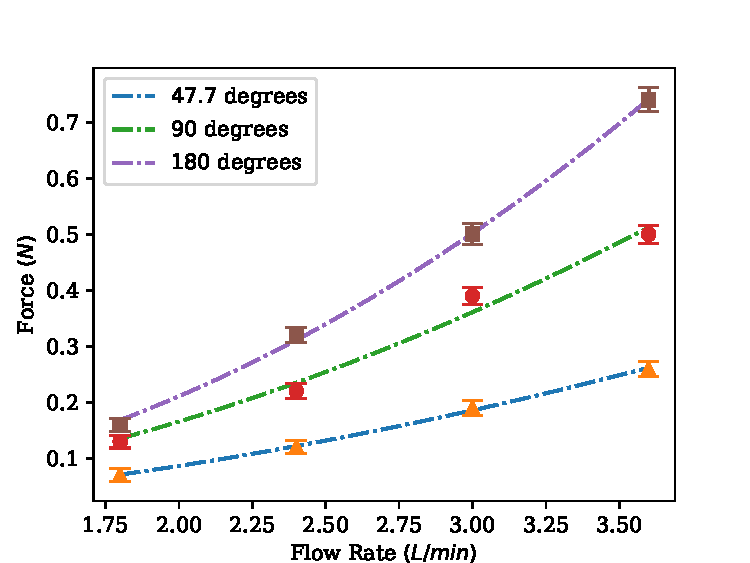
\includegraphics[width=3.25in]{Force vs. Volume Flow Rate (Chase)/plot0.pdf}} 
   \subfloat[3.28mm nozzle]{\label{fig:subB}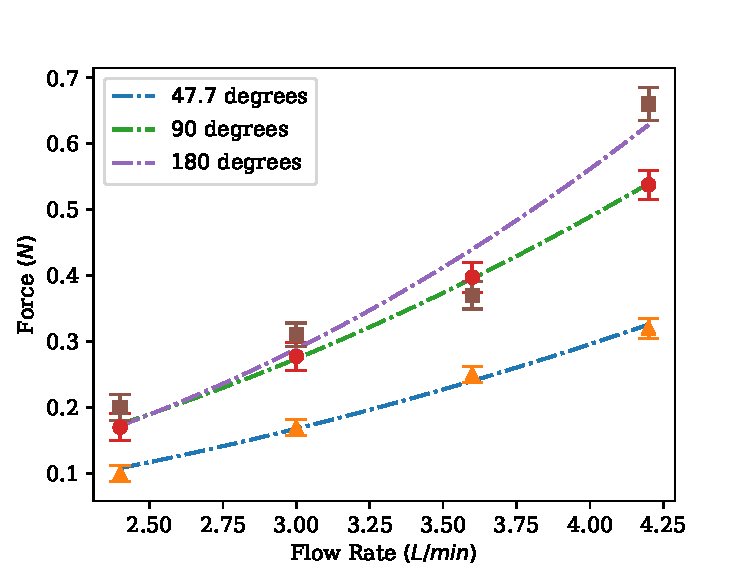
\includegraphics[width=3.25in]{Force vs. Volume Flow Rate (Chase)/plot5.pdf}} \\
   \subfloat[5.25mm nozzle.]{\label{fig:subC}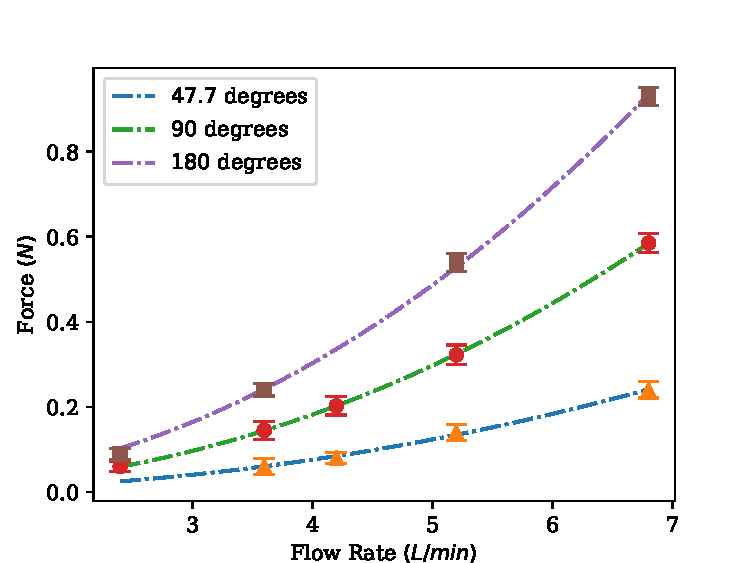
\includegraphics[width=3.25in]{Force vs. Volume Flow Rate (Chase)/plot10.pdf}}
   \subfloat[6.35mm nozzle.]{\label{fig:subD}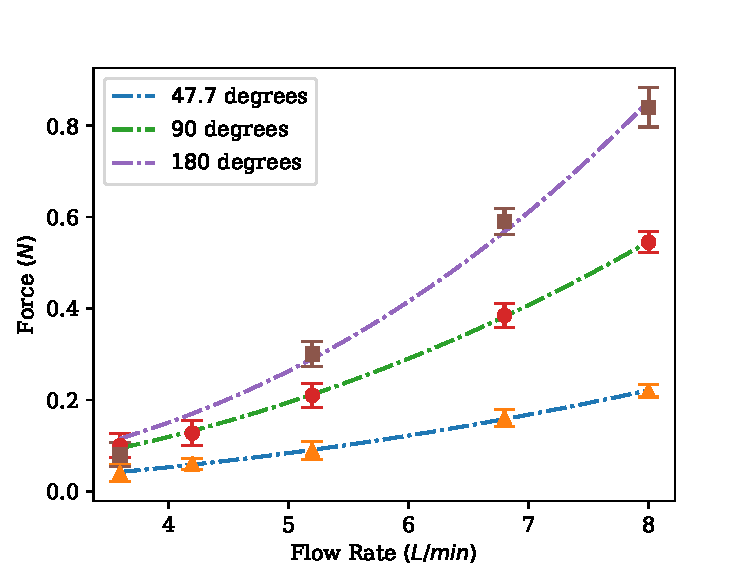
\includegraphics[width=3.25in]{Force vs. Volume Flow Rate (Chase)/plot15.pdf}} 
   \caption{Data was taken for 4 differing nozzle sizes along with 3 different angles. Uncertainty was accounted for in the error bars for the force measurement prob.
   }
   \label{fig:t49}
\end{figure}

\begin{table}[]
\caption{Resulting power coefficients from the linear regression performed on measured data}
\ra{1.2}
    \centering
    \begin{tabular}{lcccc@{}}\toprule
        D_N (mm) & 47.7\dgr & 90\dgr & 180\dgr \\\midrule
         2.83 & 1.88 & 1.92 & 2.14\\
         3.28 & 1.97& 2.01 & 2.31\\
         5.25 & 2.17& 2.20 & 2.12\\
         6.35 & 2.07& 2.19 & 2.50  \\\bottomrule
    \end{tabular}
    
    \label{tab:my_label}
    \vspace{10pt}
\end{table}

 \begin{figure}
   \centering
   \subfloat[2.83mm nozzle.]{\label{fig:subA}\includegraphics[width=3.25in]{Force vs. Volume Flow Rate (Chase)/model2.830.pdf}} 
   \subfloat[3.28mm nozzle ]{\label{fig:subB}\includegraphics[width=3.25in]{Force vs. Volume Flow Rate (Chase)/model3.280.pdf}} \\
   \subfloat[5.25mm nozzle.]{\label{fig:subC}\includegraphics[width=3.25in]{Force vs. Volume Flow Rate (Chase)/model5.250.pdf}}
   \subfloat[6.35mm nozzle.]{\label{fig:subD}\includegraphics[width=3.25in]{Force vs. Volume Flow Rate (Chase)/model6.350.pdf}} 
   \caption{Models of the for produced by different nozzles and volumetric flow rates are presented. Error bars take into account the error uncertainty that exists due to the equipment being used.
   }
   \label{fig:t49}
\end{figure}

 \begin{figure}
   \centering
   \subfloat[Modeled data for 3.28mm nozzle.]{\label{fig:subA}\includegraphics[width=3.25in]{Force vs. Volume Flow Rate (Chase)/model3.280.pdf}} 
   \subfloat[Measured data for 3.28mm nozzle. ]{\label{fig:subB}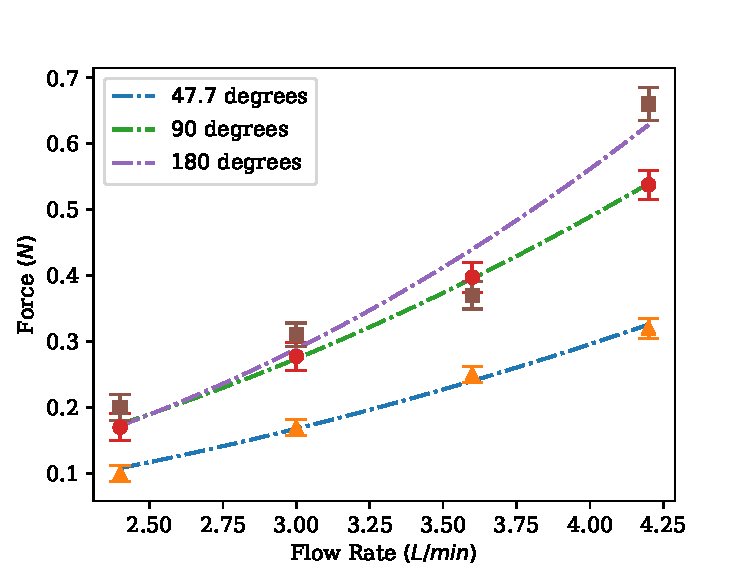
\includegraphics[width=3.25in]{Force vs. Volume Flow Rate (Chase)/plot5.pdf}} \\

   \caption{Model and measured data being compared side by side.
   }
   \label{fig:t49}
\end{figure}

\begin{table}[]
    \centering
    \caption{Measured Data and accompanying stand deviations.}
    \begin{tabular}{@{}cccccccc@{}}\toprule
    && \multicolumn{6}{c}{Target Angle}\\   \cmidrule{3-8}
    && \multicolumn{2}{c}{$47.7\dgr$} & \multicolumn{2}{c}{$90\dgr$} & \multicolumn{2}{c}{$180\dgr$}\\
    \cmidrule{3-4}  \cmidrule{5-6}  \cmidrule{7-8}
    $D_N \ (mm)$ & $\dot\vlm \ (L/m)$ & F ($N$) & $\sigma (N)$ & F ($N$) & $\sigma (N)$ & F ($N$) & $\sigma (N)$\\  \midrule
    \multirow{4}{*}{2.83} & 1.8 & 0.07 & 0.0025 & 0.013 & 0.0028 & 0.16 & 0.0032\\
    & 2.4 & 0.12 & 0.0026 & 0.22 & 0.0046 & 0.32 & 0.0049\\
    & 3 & 0.19 & 0.0048 & 0.39 & 0.0054 & 0.5 & 0.0078\\
    & 3.6 & 0.26 & 0.0047 & 0.5 & 0.0064 & 0.74 & 0.0096\\  \midrule
    \multirow{4}{*}{3.28} & 2.4 & 0.1 & 0.0034 & 0.17 & 0.009025 & 0.2 & 0.0086\\
    & 3 & 0.17 & 0.0036 & 0.2775 & 0.00925 & 0.31 & 0.0075\\
    & 3.6 & 2.5 & 0.0036 & 0.3975 & 0.010225 & 0.37 & 0.0091\\
    & 4.2 & 0.32 & 0.0055 & 0.5375 & 0.0099 & 0.66 & 0.0113\\   \midrule
    \multirow{5}{*}{5.25} & 2.4 &&& 0.06 & 0.0036 & 0.09 & 0.004\\
    & 3.6 & 0.06 & 0.0075 & 0.145 & 0.00975 & 0.24 & 0.0051\\
    & 4.2 &&& 0.2025 & 0.009425 &&\\
    & 5.2 & 0.14 & 0.0079 & 0.3225 & 0.0104 & 0.54 & 0.009\\
    & 6.8 & 0.24 & 0.008 & 0.585 & 0.009825 & 0.93 & 0.0089\\   \midrule
    \multirow{5}{*}{6.35} & 3.6 & 0.04 & 0.0076 & 0.1 & 0.0122 & 0.08 & 0.0121\\
    & 4.2 &&& 0.1275 & 0.01275 &&\\
    & 5.2 & 0.09 & 0.0087 & 0.21 & 0.0122 & 0.3 & 0.0126\\
    & 6.8 & 0.16 & 0.0076 & 0.385 & 0.0123 & 0.59 & 0.0131\\
    & 8 & 0.22 & 0.0045 & 0.545 & 0.0102 & 0.84 & 0.0209\\
    \bottomrule
    \end{tabular}
    \label{data}
\end{table}

% Assignments
% Zach - Trends of force versus nozzle diameter
% Kenny - Trends of force versus target angle
% Mitch - Trends in relative uncertainty in the measured values and the model (only included for teams with five or six members)
%Comparing how uncertainty is different between the measured data set, and the modeled data set
% Matt - Trends in error with respect to all independent parameters
%How error behaves when looking at specific independent variables like nozzle diameter, volume flow rate....
% Chase - Discussion of overlap of error bars: trends and significance

\subsection{Zach - Force v nozzle diameter}
\begin{figure}
  \centering
  \subfloat[$47.7$\dgr]{\label{fig:subA}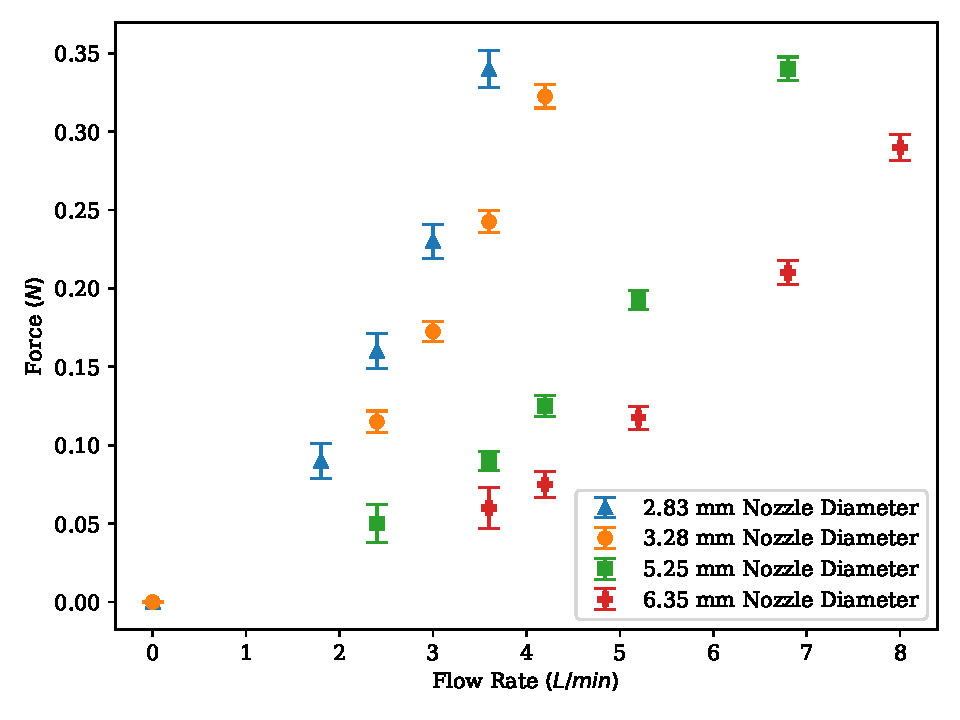
\includegraphics[width=3in]{Zach/DiscreteData.pdf}} 
  \subfloat[$90$\dgr]{\label{fig:subB}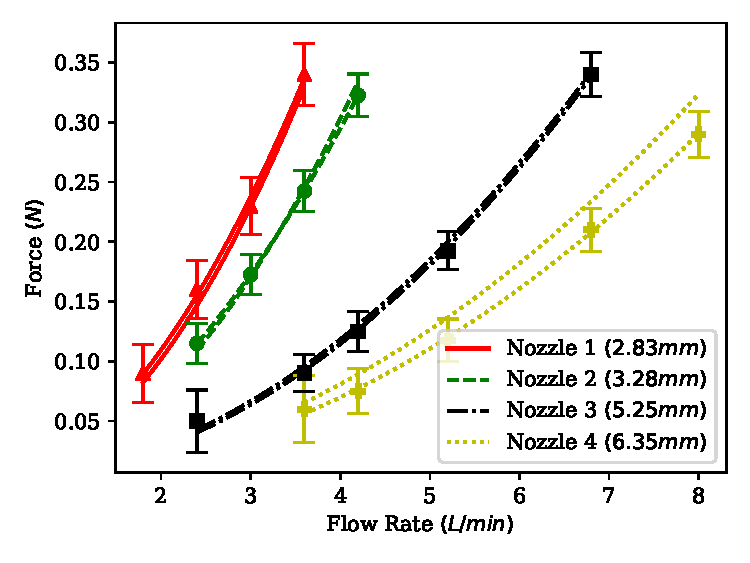
\includegraphics[width=3in]{Zach/plotFinal65.pdf}} \\
  \subfloat[$120$\dgr]{\label{fig:subC}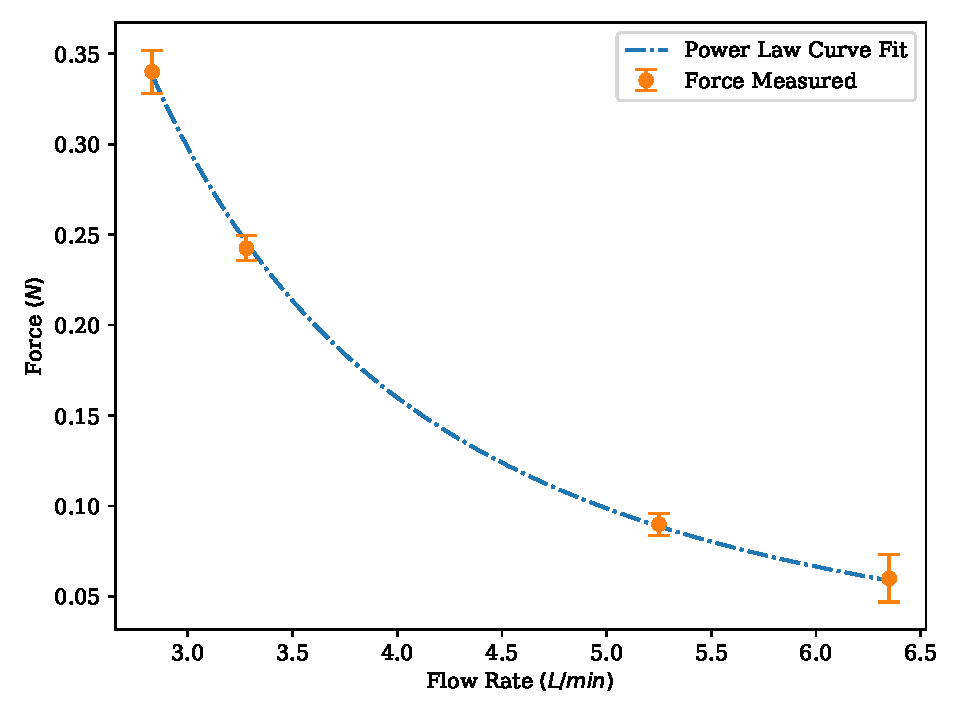
\includegraphics[width=3in]{Zach/NozzleVForce.pdf}}
%   \subfloat[$180$\dgr]{\label{fig:subD}\includegraphics[width=3in]{Zach/Combo180.pdf}} 
  \caption{Plots}
  \label{fig:Plots}
\end{figure}
\subsection{Kenny - Force v target angle}
\subsection{Mitch - relative uncertainty v measured values and model}
lllll
\subsection{Matt - Trends in error v independent parameters}
\subsection{Chase - Overlapping error bars, trends and significance}


\end{document}